\subsection{Calculate Unique Targets}
\label{sec:ui_associate_tr}

This task allows creation of UTNs (Unique Target Numbers) and target report association based on Mode S Addresses, Mode A/C codes and position information. \\

Each target found is identified by a UTN, and groups together all reference/tracker/sensor target reports (which can) be associated to this target.

Please note that if usage of UTNs is not needed, these step does not have to be performed. If usage of the evaluation feature is wanted, running this task is required. \\

\begin{figure}[H]
  \center
    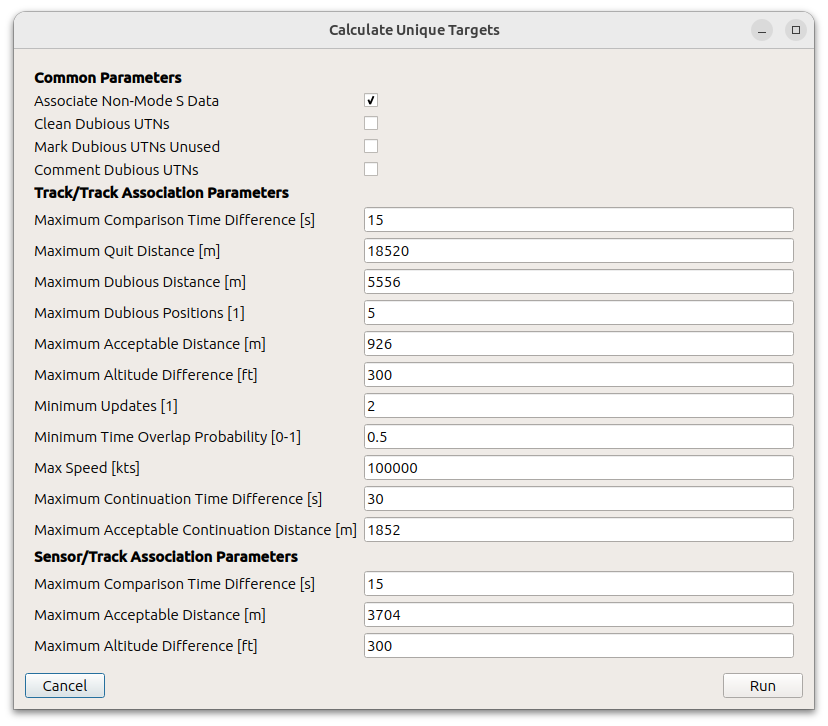
\includegraphics[width=16cm]{figures/tr_association_config.png}
  \caption{Calculate Unique Targets Configuration}
\end{figure}

The configuration of the task requires knowledge of the internals of how the associations are made. As a brief description, the following steps are performed:

\begin{itemize}
\item Delete all previously existing associations
\item Load all target reports, per data source
\item Add UTNs based on Reference (RefTraj) data sources
\item Add UTNs based on Tracker data sources
\item Add UTNs based on remaining sensor data sources
\end{itemize}
\ \\

Common parameters:
\begin{table}[H]
  \center
  \begin{tabularx}{\textwidth}{ | l | l | X |}
    \hline
    \textbf{Parameter} & \textbf{Default} &  \textbf{Description} \\ \hline
    Associate Non-Mode S Data & true & Whether Mode A/C code \& position based association should be performed \\ \hline
    Clean Dubious UTNs & true & Whether UTNs with dubious movement should have non-Mode S target report removed \\ \hline
    Mark Dubious UTNs Unused & false & Whether UTNs with dubious movement should be marked as such \\ \hline
    Comment Dubious UTNs & true & Whether UTNs with dubious movement should be commented as such \\ \hline
  \end{tabularx}
\end{table}
\ \\

The other parameters are discussed in following sub-sections.

\subsubsection{Reference/Tracker UTN Creation}

Track/Track Association Parameters:
\begin{table}[H]
  \center
  \begin{tabularx}{\textwidth}{ | X | l | X |}
    \hline
    \textbf{Parameter} & \textbf{Default} &  \textbf{Used In} \\ \hline
    Maximum Comparison Time Difference [s] & 15.0 & All (maximum time delta for any code/position comparison) \\ \hline
    Maximum Quit Distance [m] & 18520 & Target/target association \\ \hline
    Maximum Dubious Distance [m] & 5556 & Target/target association \\ \hline
    Maximum Dubious Positions [1] & 5 & Target/target association \\ \hline
    Maximum Acceptable Distance [m] & 926 & Target/target association \\ \hline
    Maximum Altitude Difference [ft] & 300 & Target/target association \\ \hline
    Minimum Updates [1] & 2 & Target/target association \\ \hline
    Minimum Time Overlap Probability [0-1] & 0.5 & Target/target association \\ \hline
    Max Speed [kts] & 100000 & Dubious target detection \\ \hline
    Maximum Continuation Time Difference [s] & 30 & Track continuation \\ \hline
    Maximum Acceptable Continuation Distance [m] & 1852 & Track continuation \\ \hline
  \end{tabularx}
\end{table}
\ \\

The following steps are performed for each Reference/Tracker data source:
\begin{itemize}
\item Per-source target creation
\begin{itemize}
\item Create new list of targets based on
\begin{itemize}
\item Track number
\item Mode S address
\item Mode A/C, time difference, position difference (track continuation)
\end{itemize}
\item Find dubious targets (dubious target detection)
\item Clean dubious targets (if configured)
\end{itemize}
\begin{itemize}
\item Per-source target to common target association (target/target association)
\item Score-based approach
\item Associates new per-source targets to existing targets based on
\begin{itemize}
\item Mode S address
\item Time overlap
\item Mode A code(s) similiarity (only if minimum time overlap is given)
\item Mode C code(s) similiarity (only if Mode A similiarity is given)
\item Position similiarity (only if Mode A/C similiarity is given)
\end{itemize}
\end{itemize}
\end{itemize}
\ \\

After creating targets for all Reference/Tracker data sources:
\begin{itemize}
\item Find dubious targets
\item Clean dubious targets (if configured)
\item Mark/comment dubious targets (if configured)
\end{itemize}
\ \\

The exact method discussion will be added at a later time, since the algorithms will be improved to include position accuracy information (error standard deviation etc.) in the near future. \\

After these steps, for each target which can be created by the simple score-based association method will be used to additionally associate sensor target reports (non Reference/Tracker based target reports), as discussed in the next section.

\subsubsection{Sensor UTN Creation}

Sensor/Track Association Parameters:
\begin{table}[H]
  \center
  \begin{tabularx}{\textwidth}{ | l | l | X |}
    \hline
    \textbf{Parameter} & \textbf{Default} &  \textbf{Description} \\ \hline
    Maximum Comparison Time Difference [s] & 15 & Maximum time delta for any code/position comparison \\ \hline
    Maximum Acceptable Distance [m] & 3704 & Maximum position difference \\ \hline
    Maximum Altitude Difference [ft] & 300 & Maximum altitude difference \\ \hline
  \end{tabularx}
\end{table}

The following steps are performed for each sensor data source:
\begin{itemize}
\item Find possible target in existing target list based on
\begin{itemize}
\item Mode S address
\item Mode A code similiarity (if present)
\item Mode C code similiarity (if present)
\item Position similiarity
\end{itemize}
\item If a matching target is found, the best match is used for association
\item If no matching target is found
\begin{itemize}
\item If the target report has Mode S address, a new target is created
\item Otherwise no association is made
\end{itemize}
\end{itemize}
\ \\

\subsubsection{Dubious Targets}

The dubious target check is solely based on a simple maximum speed given all associated Reference/Tracker target reports. It should be used to detect/mark possibly wrong associations, to investigate such targets later and, if possible, resolve such issues using different parameter values. \\

Please note that in a special case where target reports from difference Reference/Tracker source are very close in time this check can generate a large number of false positives and should be disabled. For this reason the default value was set to a disproportionately high value.

\subsubsection{Discussion}

The user should be aware that, while this association feature is quite an improvement over the previous method, it is still somewhat limited. It strongly depends on the correctness of Mode S addresses, as well as the Reference/Tracker information (track number, secondary information and position information). If the mentioned information is erroneous, the made association will be sub-optimal or plainly wrong. \\

For the Sensor UTN Creation, the correctness of the associations strongly depends again on the Mode S address as well as the quality of the assocations made in the Reference/Tracker UTN Creation. \\

Also, for association of non Mode S sensor target reports a trade-off has to be made in the 'Maximum Acceptable Distance' parameter, especially if they are primary-only. It should be set within the limits of Reference/Tracker error plus maximum sensor error (which can still include radar bias') and the used target separation minima. This is of course not well-suited for strongly different sensors accuracies and seperations (e.g. when mixing ground and air surveillance data). \\

\subsubsection{Running}

To run the task, click the 'Run' button. After the assocations are saved, the task is done:

\begin{figure}[H]
  \center
    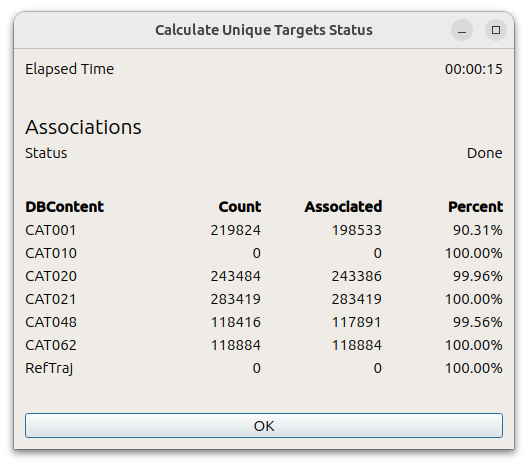
\includegraphics[width=10cm]{figures/tr_association_done.png}
\end{figure}
